\newpage
\section{ZFOURGE Observational Results}
To confirm that the galaxies chosen for this project accurately reflected the redshift range available in ZFOURGE, redshift distributions of the entire ZFOURGE survey and the chosen subsample were created (See Figure \ref{fig:redshifts}) were generated. The subsample was created through bootstrapping to estimate the relative shape of the distribution.  This allowed us to examine the redshift distribution within the full ZFOURGE Survey and the specific subsample used in this study. Both distributions are left-skewed and have a median redshift of 1.06. Although the overall shapes of the two distributions are comparable, the subsample contains a significantly lower number of galaxies at the higher redshift end of the distribution.
\begin{figure}[h]
    \centering
    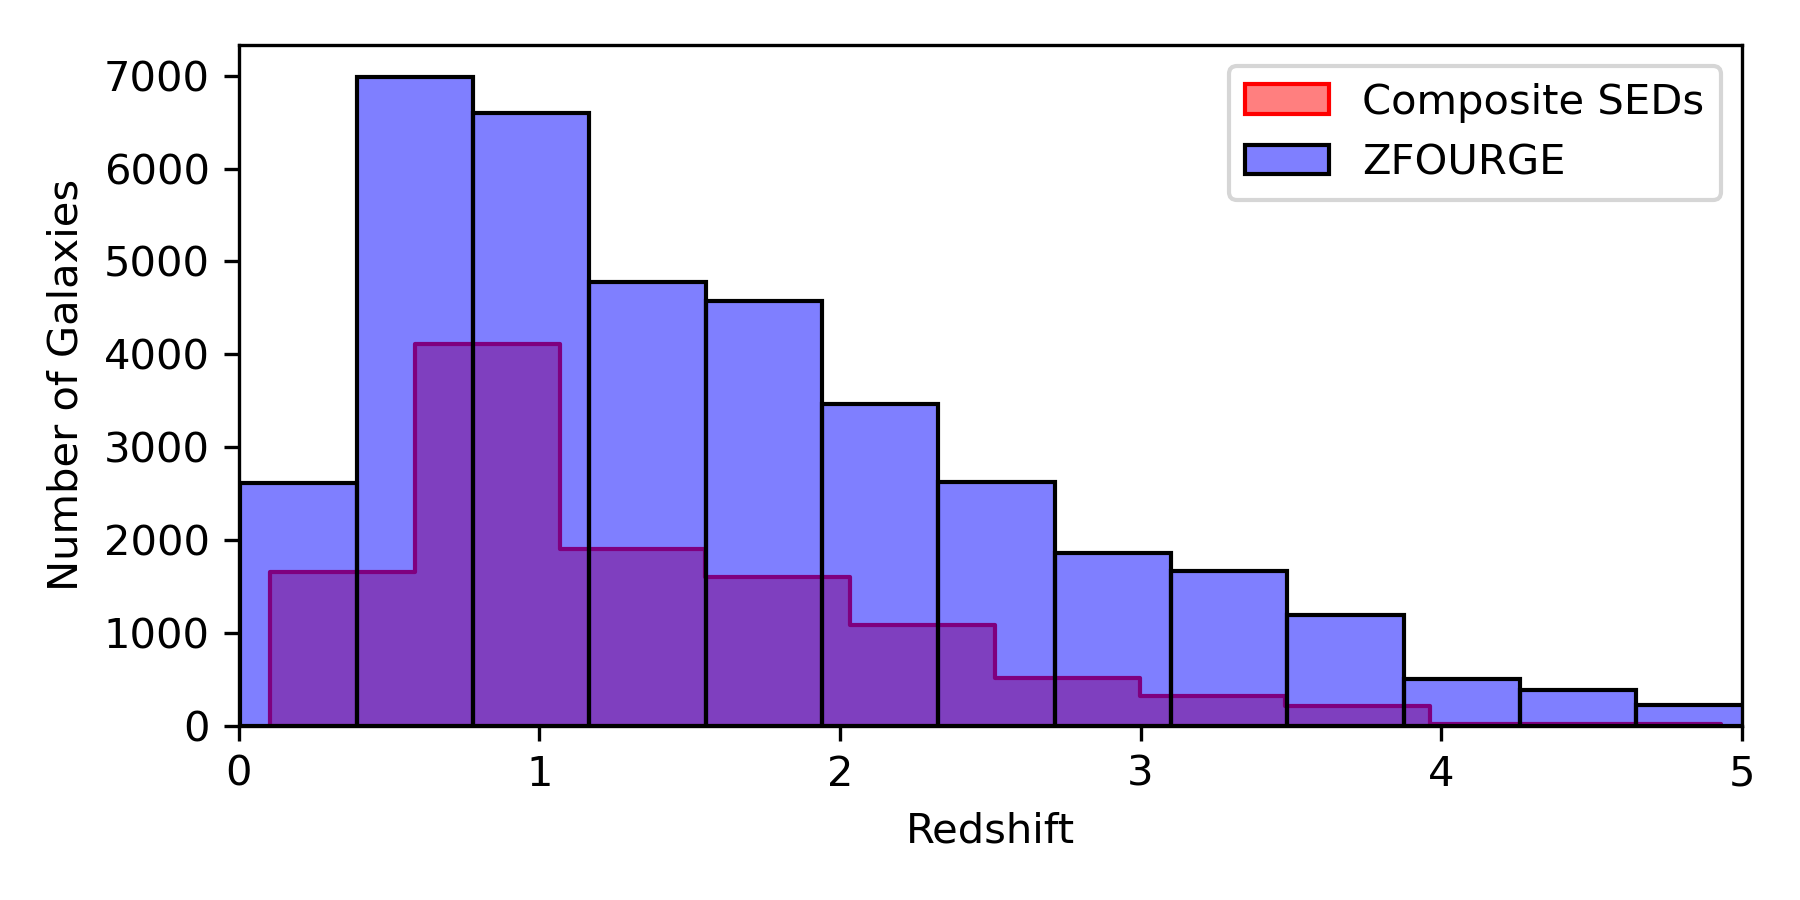
\includegraphics[width=0.60\linewidth]{Images/TheoreticalModelPlots/ZFOURGE_obsevational_composites_fluxesType1AGN_redshift_distribution.png}
    \caption{Redshift Distribution for both the public ZFOURGE survey and the resampled data used in this thesis.}
    \label{fig:redshifts}
\end{figure}
\subsection{EAZY SED Fitting}
Using EAZY, photometric data from the ZFOURGE survey was used to produce 11449 unique SEDs across the CDFS, COSMOS and UDS fields (See Figure \ref{fig:ZFOURGE-EAZY-SEDFit}). Examining these galaxies reveals that the de-redshifting process was successful and that the SEDs are in the restframe. This result is evident in the alignment of their emission lines, and the Lyman break at 912$\AA$.
\begin{figure}[h!]
    \centering
    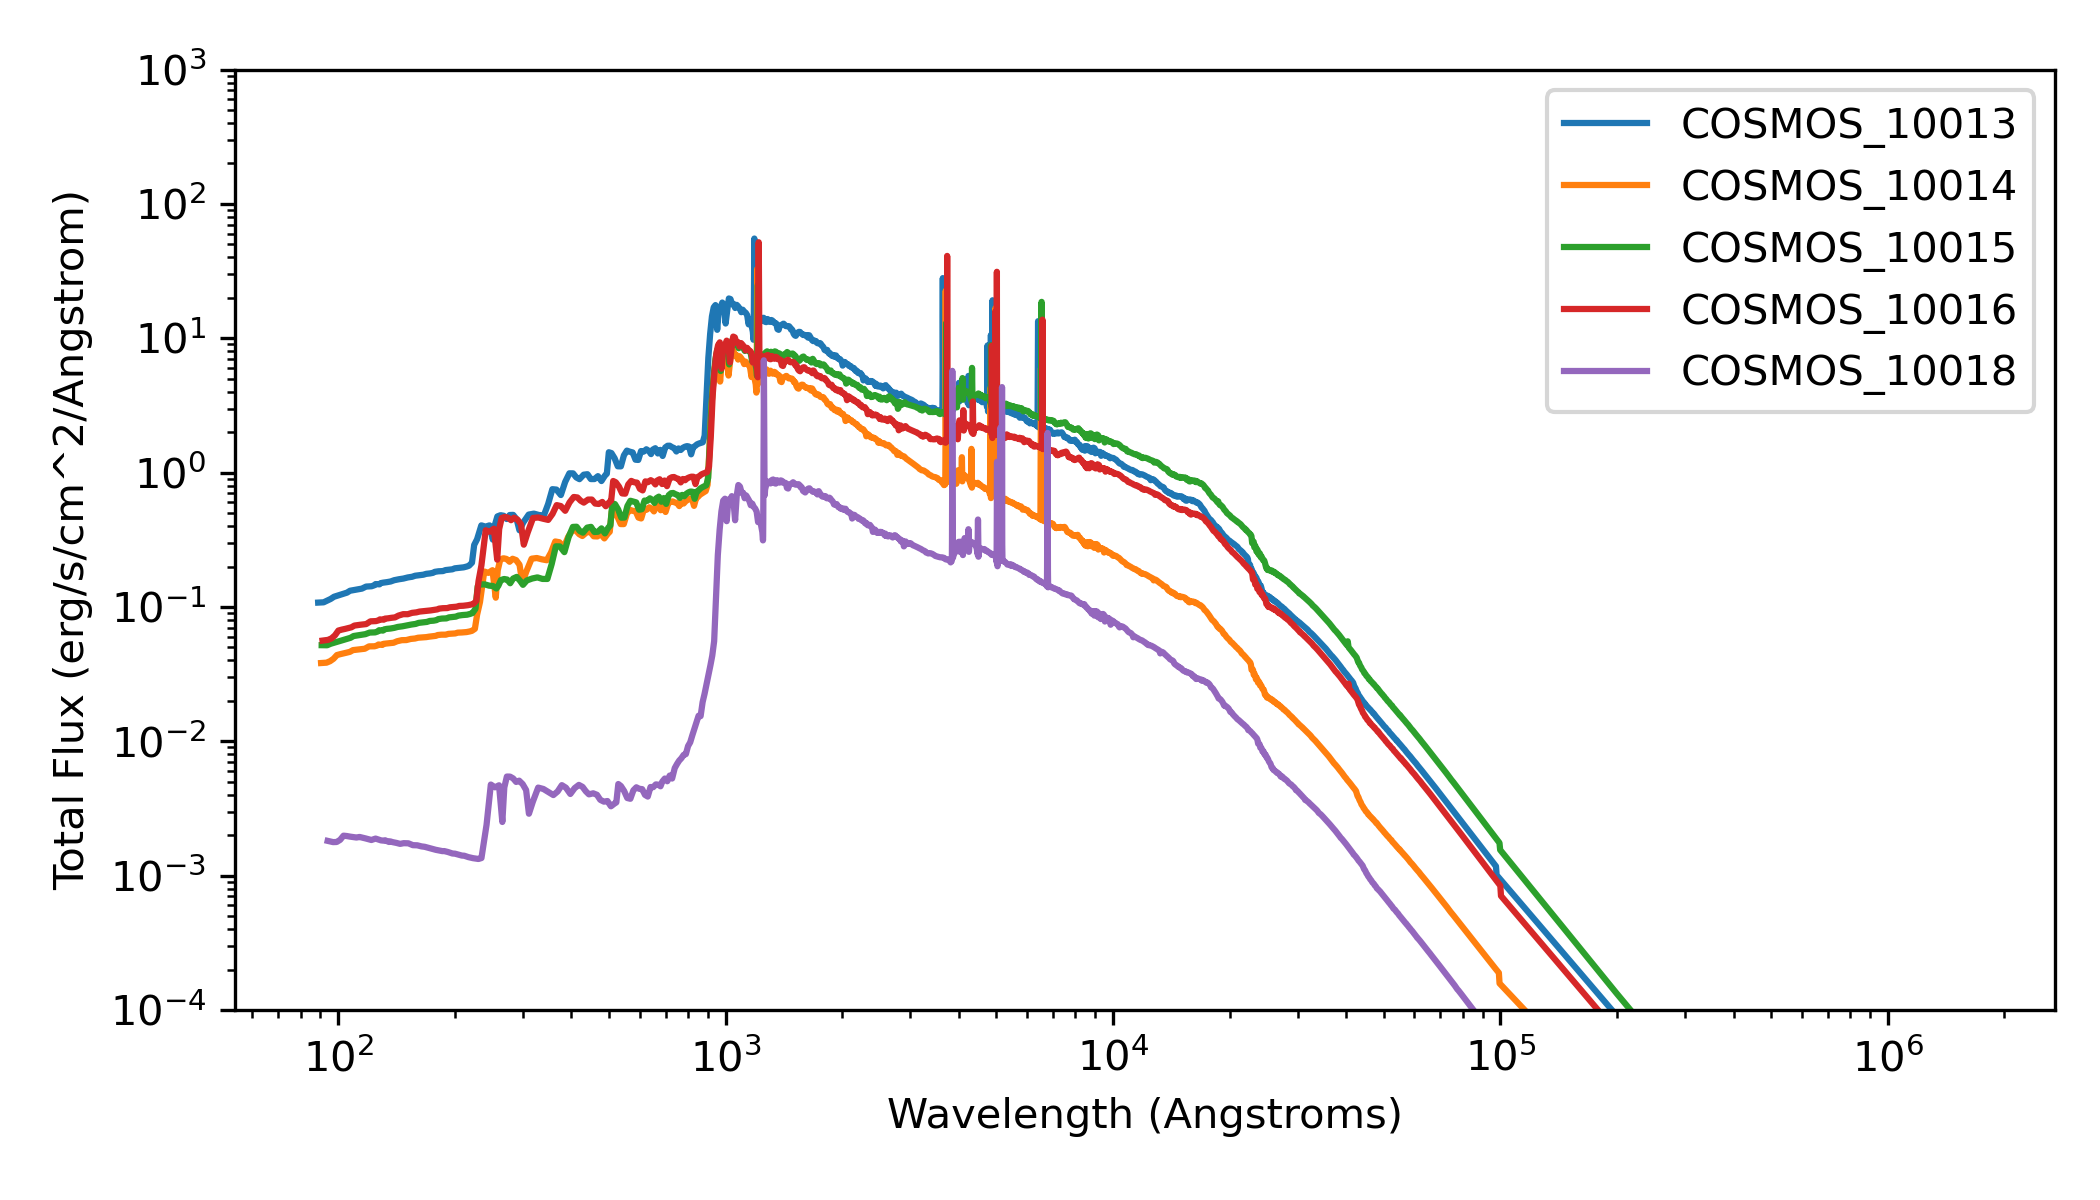
\includegraphics[width=0.60\textwidth]{Images/ZFOURGE_SED_Templates_EAZYFIT.png}
    \caption{SEDs of restframe galaxies that have been fit using EAZY. The galaxies shown have been shifted into the restframe using their photometric redshift, which is available from the ZFOURGE survey.}
    \label{fig:ZFOURGE-EAZY-SEDFit}
\end{figure}
\newpage
\subsubsection{EAZY Colour Space Diagrams}
 As this sample contains a large sample size (n=11449), this is far more representative of a true photometric survey as it allows for exponentially more sources to be investigated than the GALSEDATLAS templates (n=129). Once again, mean vector offsets were computed for the observational data in each colour space (refer to Table \ref{tab:combined_vectoroffset}). We see a systematic shift in the IRAC colour space for both composite sets, similar to what was observed previously. Interestingly, there are also increases in vector offsets for both ugr and UVJ type 1 composites, but with much lower values, up to a maximum of 0.24 and 0.13 dex, respectively. 
\begin{table}[h!]
    \centering
    \begin{tabular}{l|cc|cc|cc} 
        \hline
        \textbf{AGN Contribution (\%)} & \multicolumn{2}{c|}{\textbf{IRAC}} & \multicolumn{2}{c|}{\textbf{ugr}} & \multicolumn{2}{c}{\textbf{UVJ}} \\
        & \textbf{Type 1} & \textbf{Type 2} & \textbf{Type 1} & \textbf{Type 2} & \textbf{Type 1} & \textbf{Type 2} \\
        \hline
        10  & 0.12 & 0.17 & 0.09 & 0.00 & 0.02 & 0.00 \\
        20  & 0.19 & 0.26 & 0.13 & 0.00 & 0.03 & 0.00 \\
        30  & 0.25 & 0.33 & 0.16 & 0.00 & 0.05 & 0.00 \\
        40  & 0.29 & 0.39 & 0.17 & 0.00 & 0.06 & 0.00 \\
        50  & 0.33 & 0.44 & 0.19 & 0.00 & 0.08 & 0.00 \\
        60  & 0.36 & 0.48 & 0.20 & 0.00 & 0.09 & 0.00 \\
        70  & 0.38 & 0.51 & 0.21 & 0.00 & 0.10 & 0.00 \\
        80  & 0.40 & 0.54 & 0.22 & 0.00 & 0.11 & 0.00 \\
        90  & 0.42 & 0.57 & 0.23 & 0.00 & 0.12 & 0.00 \\
        100 & 0.44 & 0.60 & 0.24 & 0.00 & 0.13 & 0.00 \\
        \hline
    \end{tabular}
    \caption{Mean Vector Offsets for EAZY composite sources in multiple colour spaces}
    \label{tab:combined_vectoroffset}
\end{table}
Figure \ref{fig:ZFOURGE-EAZY-UVJ} displays the UVJ diagram for the ZFOURGE colours fitted using EAZY. The density plot reveals a substantial concentration of points within the star-forming region of this diagram. As AGN contribution increases, sources on the outer edge of this density plot, especially those in the quiescent region, gradually move towards the region of highest density. This migration also leads to a decrease in quiescent and dusty fractions, accompanied by a corresponding increase in the star-forming fraction. This process mirrors the observations made using the GALSEDATLAS templates in section 6.1.  
\begin{figure}[h]
    \centering
    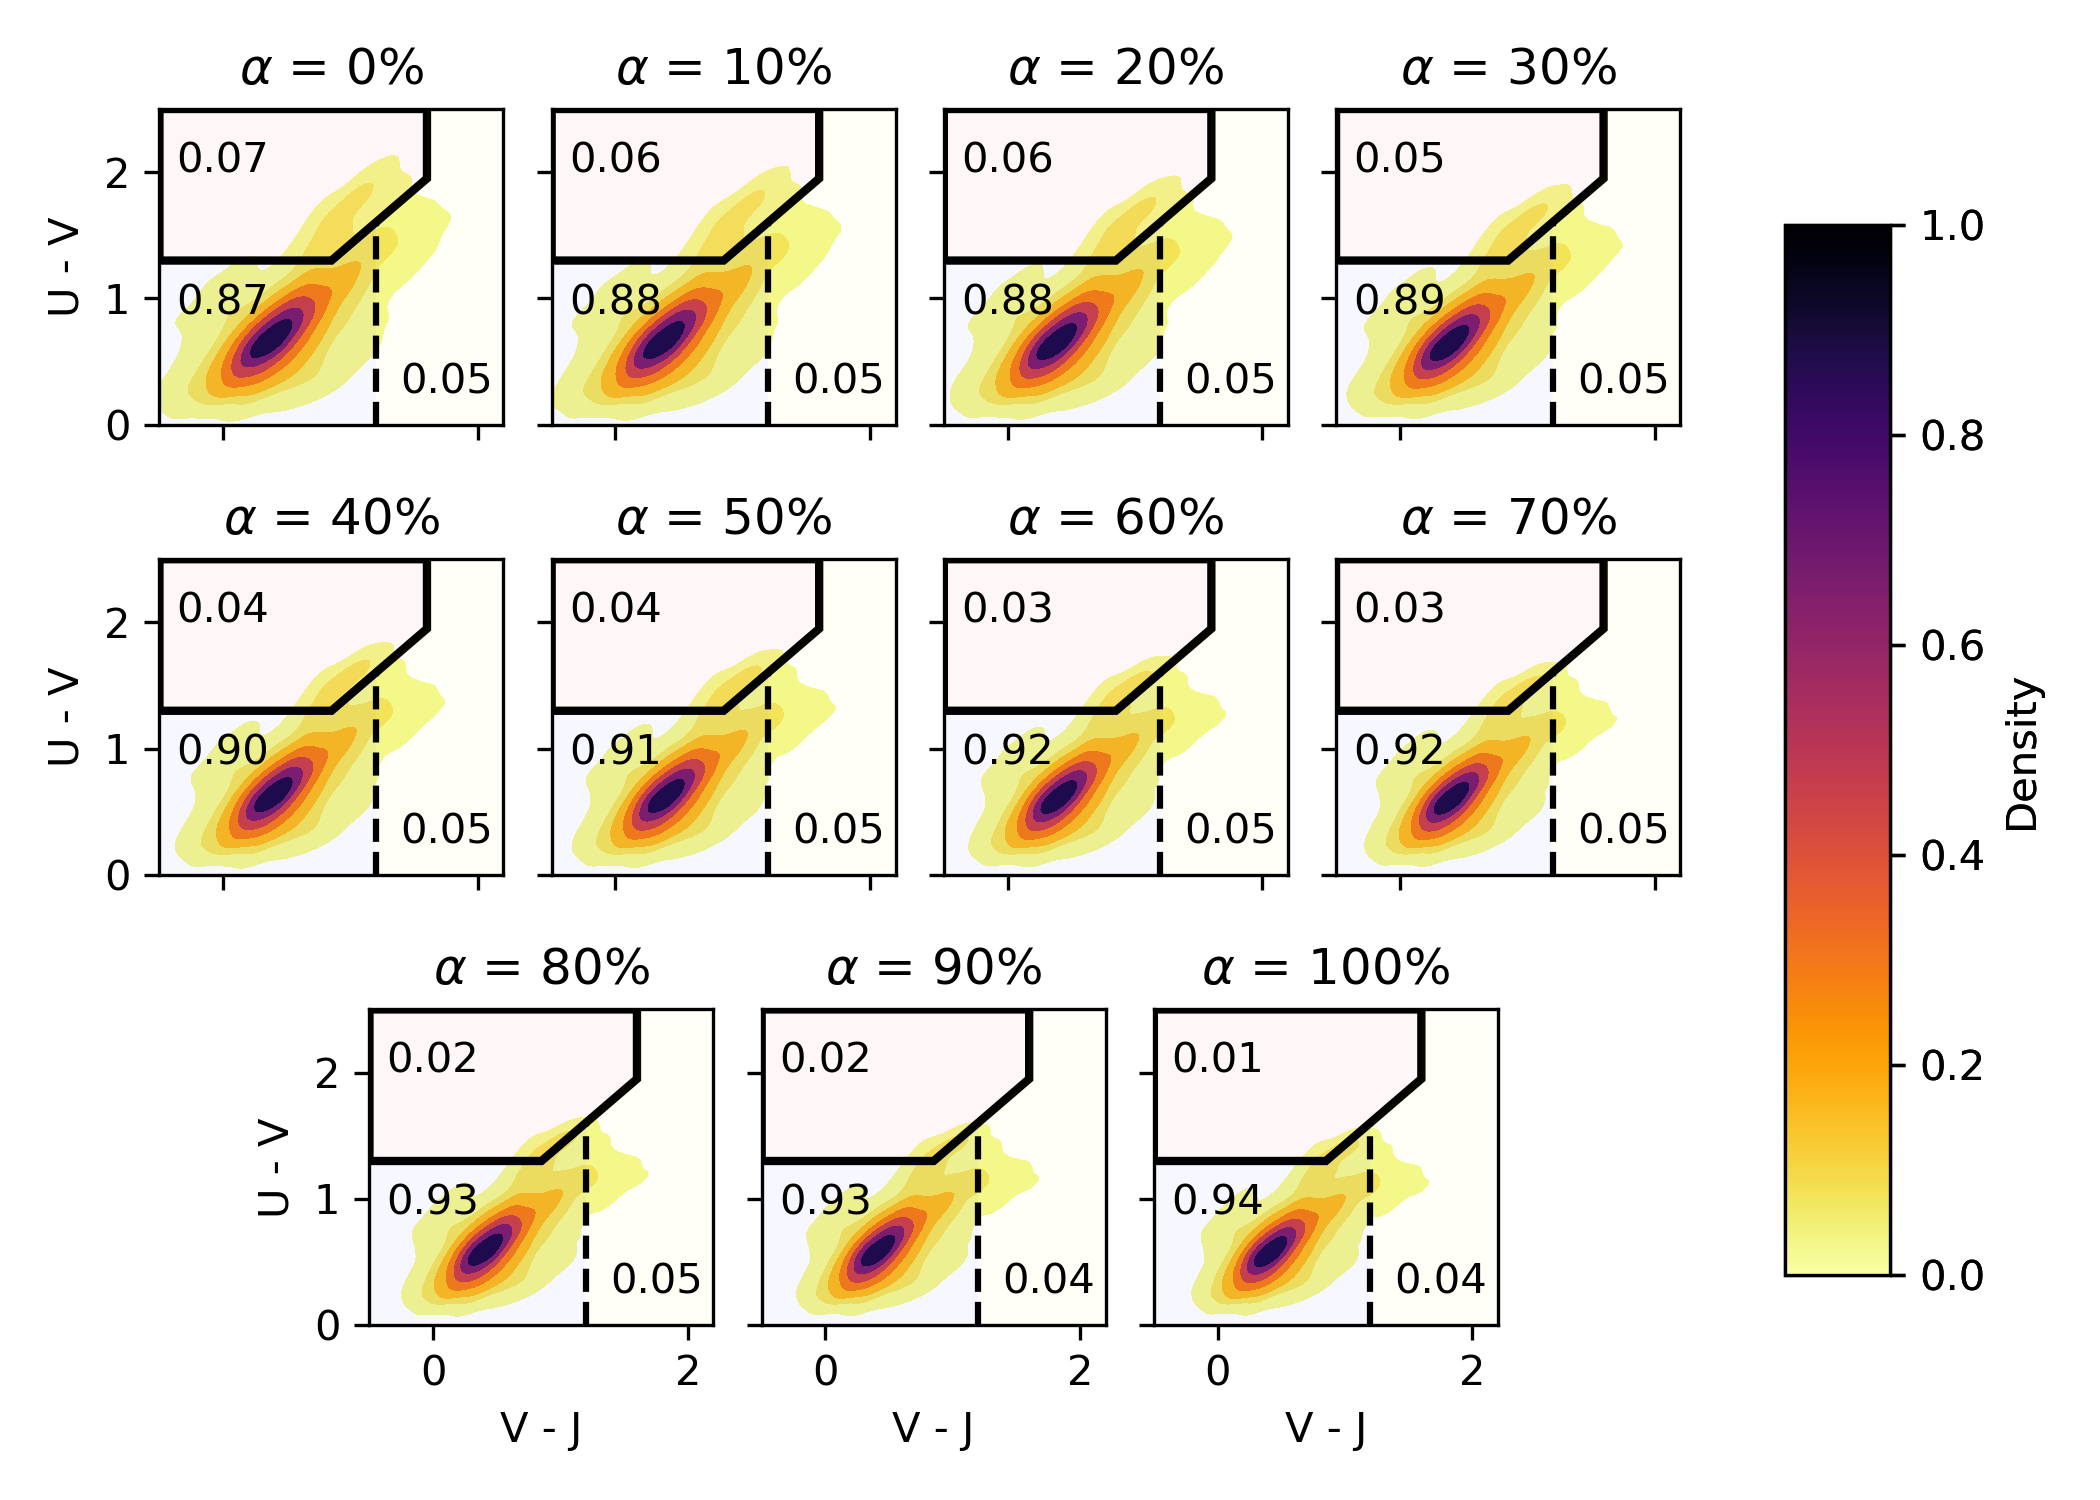
\includegraphics[width=0.6\linewidth]{Images//TheoreticalModelPlots/UVJ_evolution_Type1AGN_ZFOURGE_0_5.png}
    \caption{Density plot of Type 1 AGN composites on a UVJ diagram, demonstrating the shift from quiescent to star-forming regions with increasing AGN contribution. }
    \label{fig:ZFOURGE-EAZY-UVJ}
\end{figure}
\\The observed over-density within the star-forming region of Figure \ref{fig:ZFOURGE-EAZY-UVJ} necessitates considering region-specific colour evolution paths. Figure \ref{fig:ZFOURGE-EAZY-UVJSingleGalaxy_Comparison} illustrates this, showcasing the colour evolution of composite sources at the average position of each population of sources. Star-forming galaxies exhibit minimal colour shifts, while quiescent and dusty galaxies undergo substantial changes. While each population shifts positions, an average galaxy stays within the respective selection regions, even at high AGN contribution amounts.
\begin{figure}[h!]
    \centering
    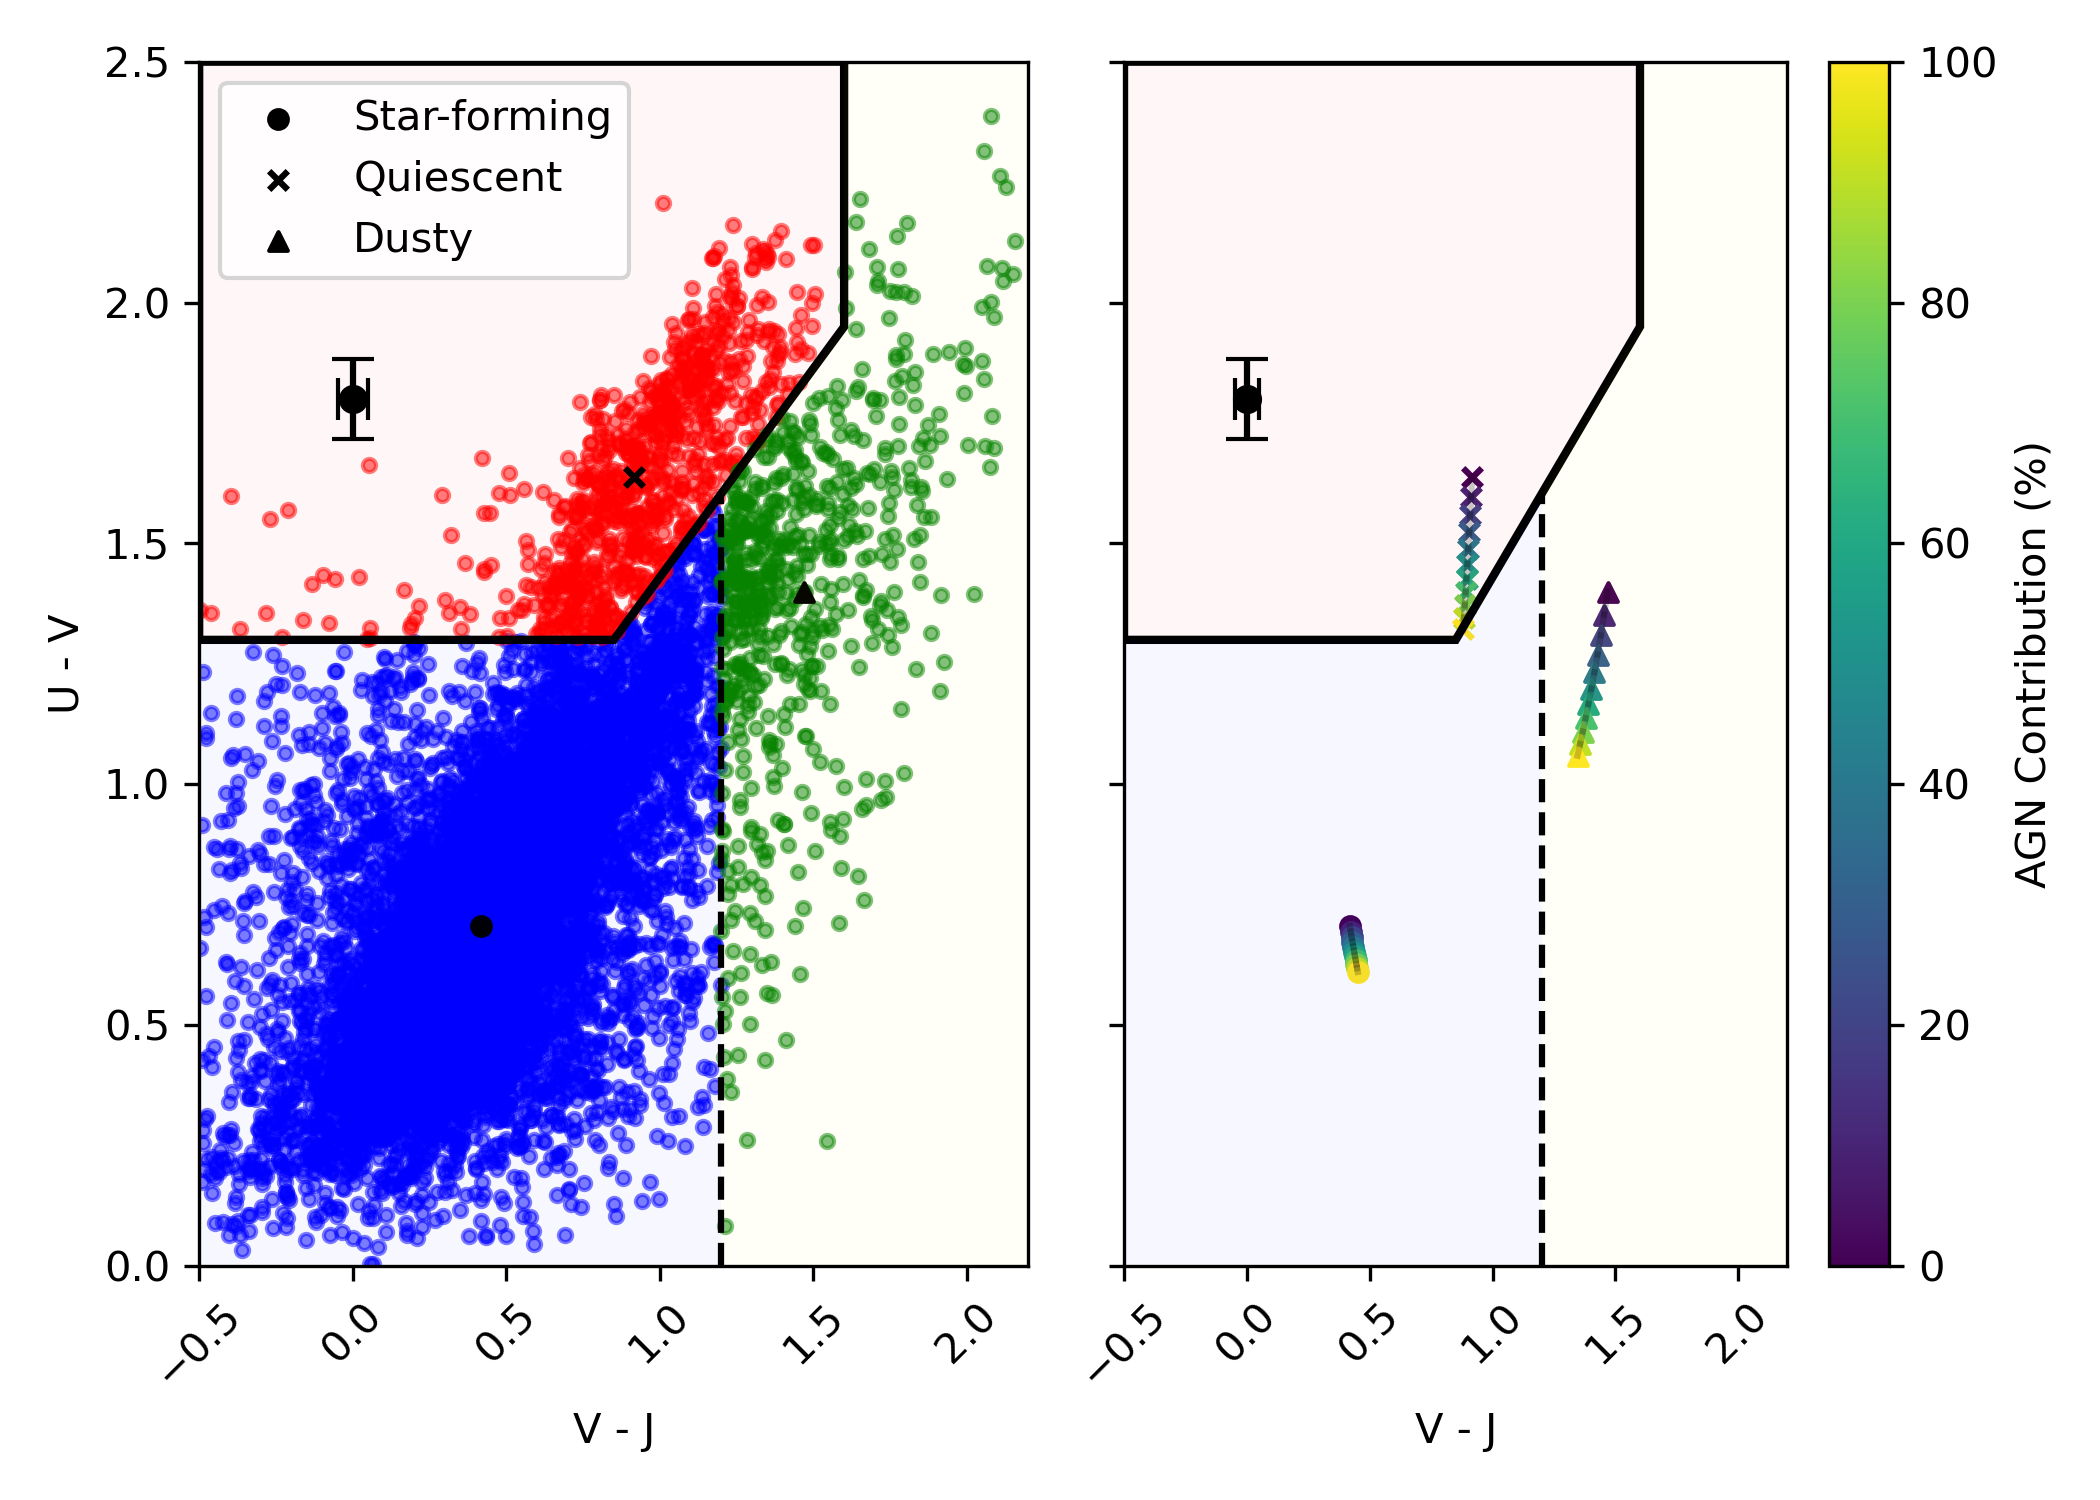
\includegraphics[width=0.65\linewidth]{Images/TheoreticalModelPlots/ZFOURGE_obsevational_composites_fluxesType1AGN_uvj_diagram_pathsubplot.png}
    \caption{The left panel shows the subsample of galaxies used in this project where the black markers represent a source that is taken to be the `average' of that population. The right panel shows the colour evolution for those sources.}
    \label{fig:ZFOURGE-EAZY-UVJSingleGalaxy_Comparison}
\end{figure} \\
We investigate the average movement for each selection region to determine if the average vector offsets are region-dependent. This is shown in Table \ref{tab:population_vectoroffset}. Our analysis reveals a distinct dependence of vector offset on the selection region. The star-forming region demonstrates a maximum shift of 0.1 dex at 100\% AGN contribution. In contrast, both the quiescent and dusty populations exhibit a more pronounced positional change, shifting by approximately 0.04 dex for every 10\% increase in AGN contribution within the composite spectra. The increase in AGN contribution causes a large increase in both the quiescent and dusty populations up to a maximum offset of 0.32 and 0.36 dex, respectively, a value far greater than what was obtained and presented in Table \ref{tab:combined_vectoroffset}.
% \begin{table}[h!]
%     \centering
%     \begin{tabular}{l|c|c|c}
%         \hline
%         \textbf{AGN Contribution (\%)} & \textbf{Star-forming} & \textbf{Quiescent} & \textbf{Dusty} \\
%         \hline
%         10  & 0.01 & 0.04 & 0.05 \\
%         20  & 0.02 & 0.08 & 0.09 \\
%         30  & 0.04 & 0.12 & 0.14 \\
%         40  & 0.05 & 0.15 & 0.18 \\
%         50  & 0.06 & 0.18 & 0.21 \\
%         60  & 0.07 & 0.21 & 0.25 \\
%         70  & 0.08 & 0.24 & 0.28 \\
%         80  & 0.08 & 0.27 & 0.31 \\
%         90  & 0.09 & 0.29 & 0.34 \\
%         100 & 0.10 & 0.32 & 0.36 \\
%         \hline
%     \end{tabular}
%     \caption{Mean vector offsets for each of the selection regions in the UVJ colour space.} 
%     \label{tab:population_vectoroffset} 
% \end{table}
\begin{table}[h!]
    \centering
    \begin{tabular}{l|ccc}
        \hline
        \textbf{AGN Contribution (\%)} & \textbf{Star-forming} & \textbf{Quiescent} & \textbf{Dusty} \\
        \hline
        10  & 0.01 & 0.04 & 0.05 \\
        20  & 0.02 & 0.08 & 0.09 \\
        30  & 0.04 & 0.12 & 0.14 \\
        40  & 0.05 & 0.15 & 0.18 \\
        50  & 0.06 & 0.18 & 0.21 \\
        60  & 0.07 & 0.21 & 0.25 \\
        70  & 0.08 & 0.24 & 0.28 \\
        80  & 0.08 & 0.27 & 0.31 \\
        90  & 0.09 & 0.29 & 0.34 \\
        100 & 0.10 & 0.32 & 0.36 \\
        \hline
    \end{tabular}
    \caption{Mean vector offsets for each of the selection regions in the UVJ colour space.} 
    \label{tab:population_vectoroffset} 
\end{table} \\
We also examined the ugr diagram for AGN contribution across redshift ranges. Figure \ref{fig:ZFOURGE-EAZY-ugrSingleGalaxy_Comparison} demonstrates the varying sensitivity of each redshift range to an increasing AGN contribution; by tracking an average source within each redshift range, it was possible to quantify the effect. Notably, the target redshift range (2.6 $<$ z $<$ 3.6) and the high-redshift range (z $>$ 3.6) exhibit significant shifts. Increasing AGN contribution pushes the target out of the selection region at 40\%. The high-redshift sources, while also significantly impacted, follow a curved trajectory that entirely avoids the selection region.
\begin{figure}[h!]
    \centering
    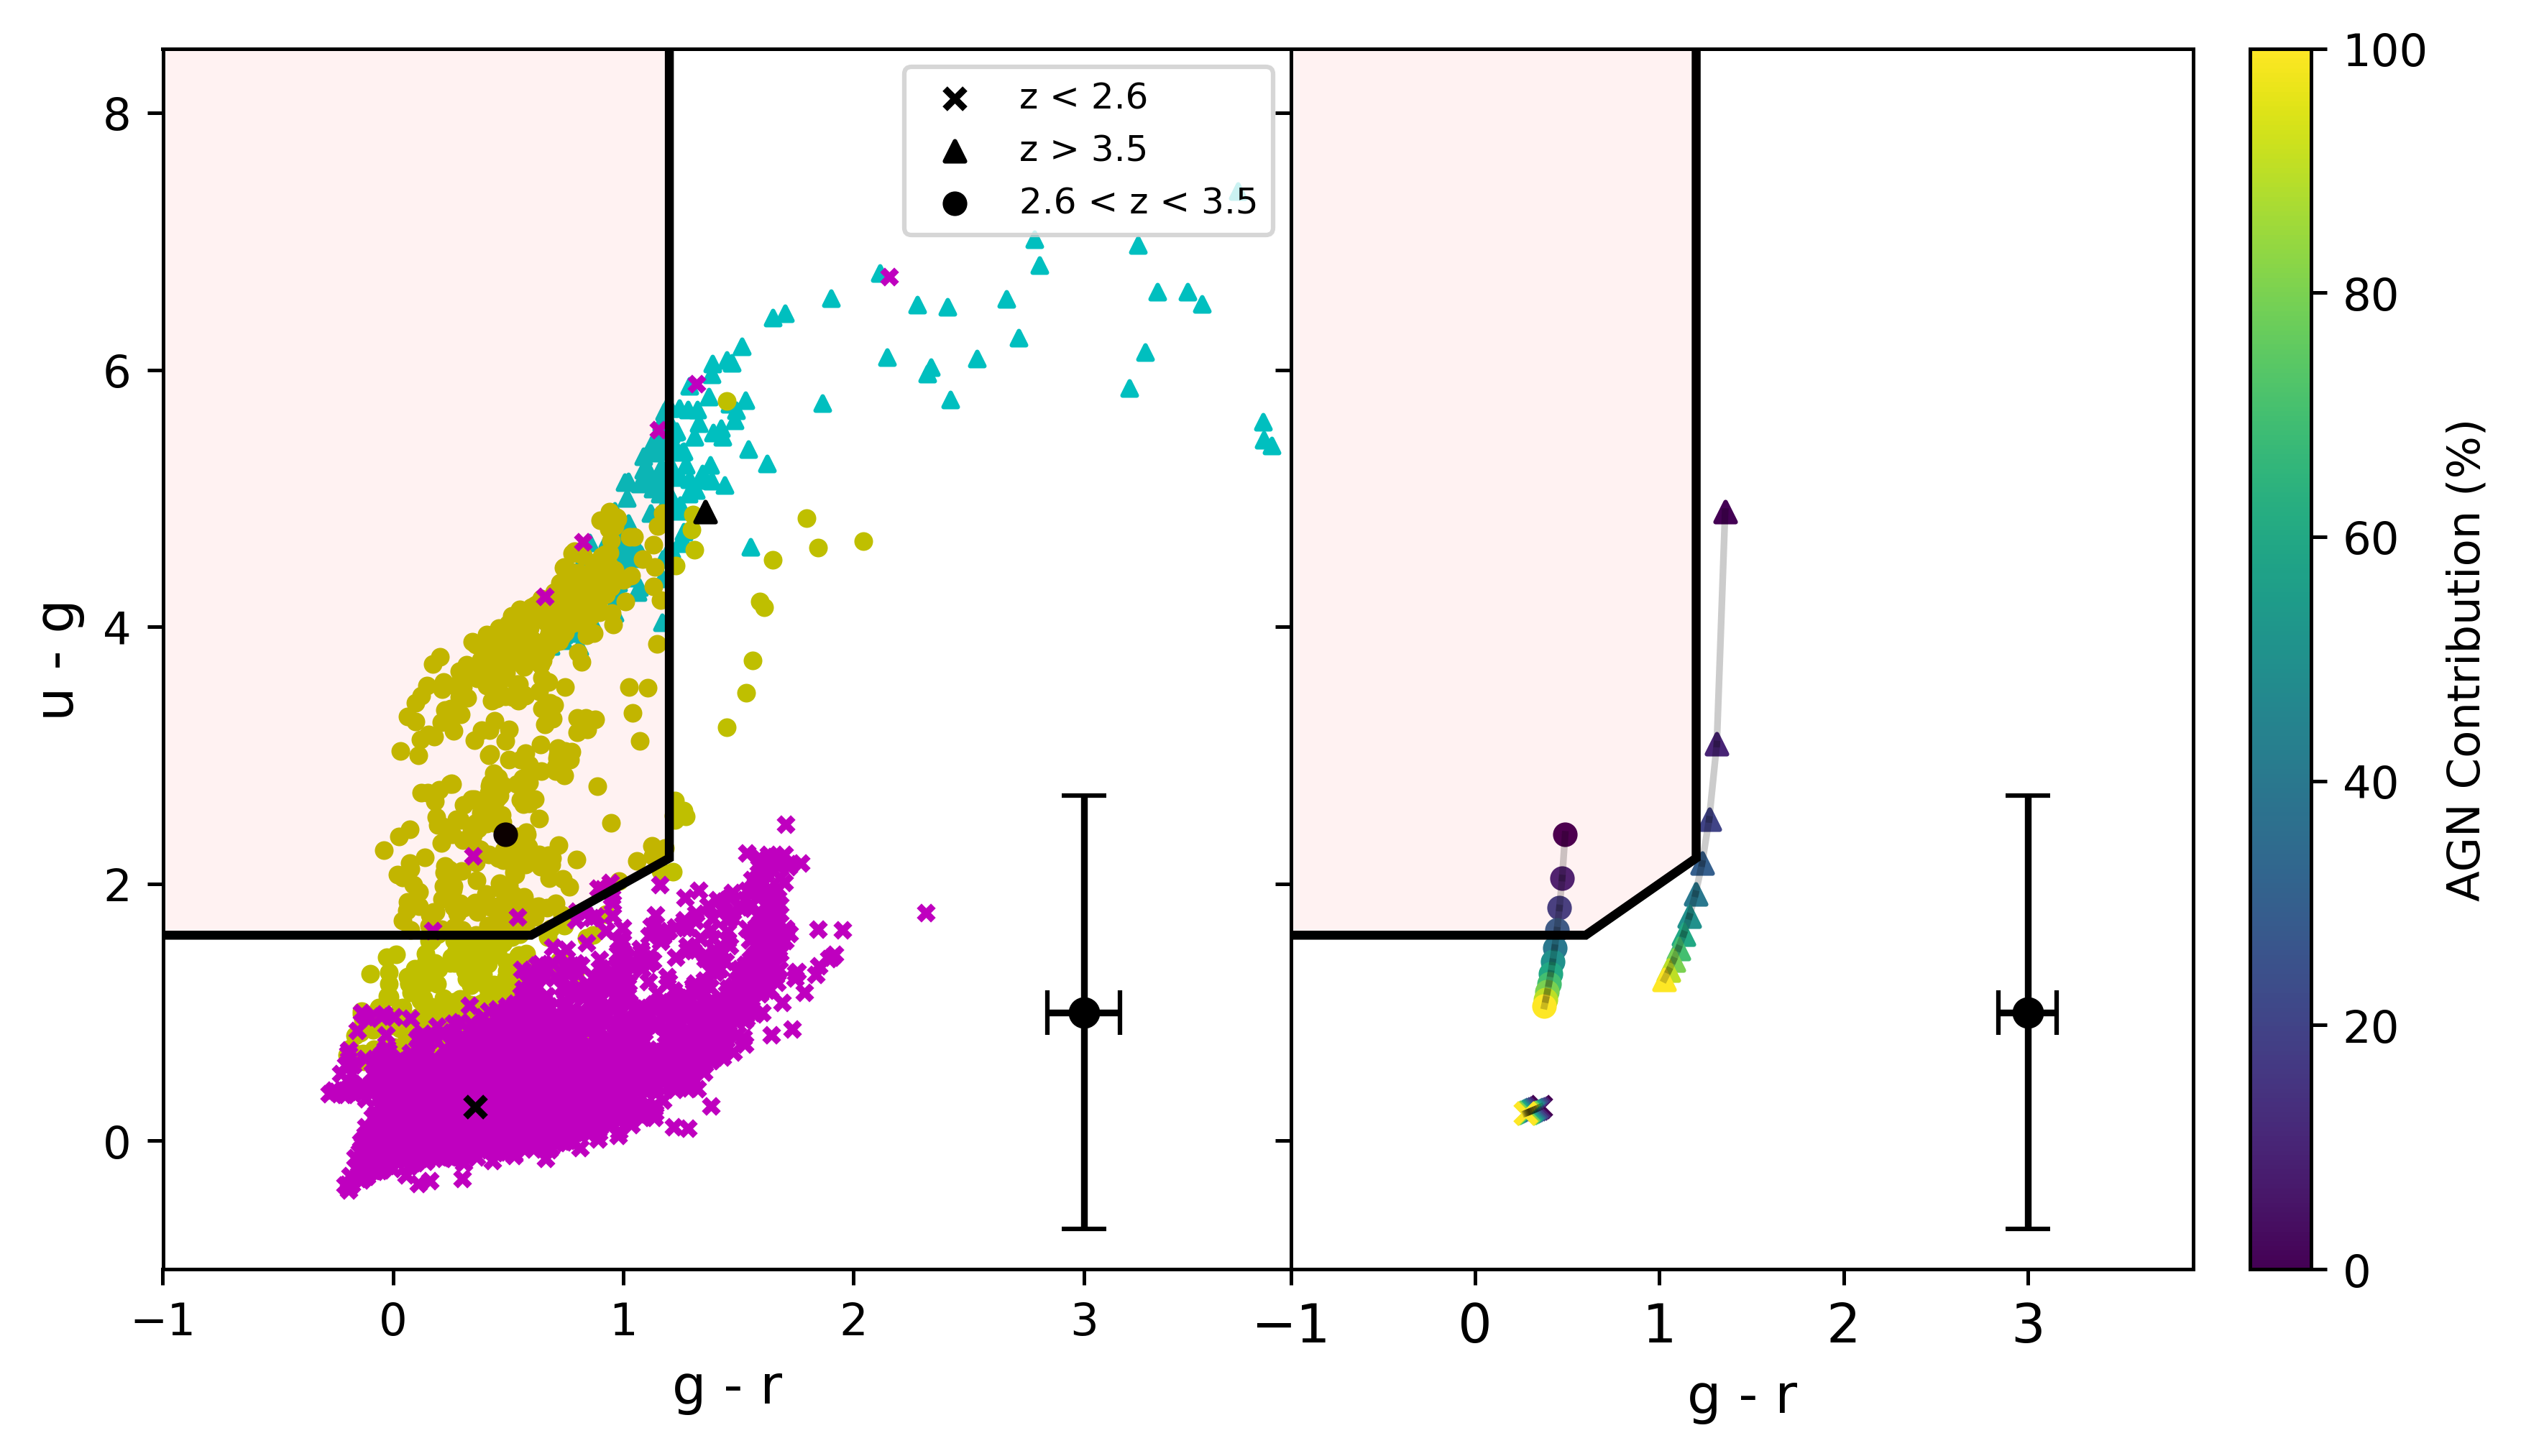
\includegraphics[width=0.65\linewidth]{Images/TheoreticalModelPlots/ugr_evolution_Type1AGN_ZFOURGE_comparison.png}
    \caption{The left panel shows the initial ugr diagram with average sources in a particular redshift range shown in black. The right panel shows the colour evolution for those sources.}
    \label{fig:ZFOURGE-EAZY-ugrSingleGalaxy_Comparison}
\end{figure}\\
We see that there is not much movement from low redshift sources while high redshift sources manage to move quite a lot throughout the selection colourspace. Table \ref{tab:population_vectoroffset_z}  quantifies this effect by showing the difference in redshift ranges for an average source within these ranges. High-redshift sources exhibit a disproportionately large effect, with movements ranging from a minimum of 1.81 dex at the lowest AGN contribution to a maximum of 3.65 dex at 100\% AGN contribution. Similarly, target redshift sources within the selection region are significantly impacted, showing vector offsets from 0.34 dex to 1.34 dex as AGN contributions increase from 10\% to 100\%. It's worth noting that while there was a significant movement for the target and high redshift range, only the high redshift range moved a distance greater than the error for this particular colour-colour diagram.
\begin{table}[h!]
    \centering
    \begin{tabular}{l|ccc}
        \hline
        \textbf{AGN Contribution (\%)} & $\mathbf{z < 2.6}$ & $\mathbf{2.6 < z < 3.6}$ & $\mathbf{z > 3.6}$ \\
        \hline
        10  & 0.02 & 0.34 & 1.81 \\
        20  & 0.03 & 0.57 & 2.40 \\
        30  & 0.04 & 0.75 & 2.74 \\
        40  & 0.05 & 0.88 & 2.98 \\
        50  & 0.06 & 0.99 & 3.15 \\
        60  & 0.07 & 1.09 & 3.29 \\
        70  & 0.08 & 1.16 & 3.41 \\
        80  & 0.08 & 1.23 & 3.50 \\
        90  & 0.09 & 1.29 & 3.58 \\
        100 & 0.10 & 1.34 & 3.65 \\
        \hline
    \end{tabular}
    \caption{Mean vector offsets for each of the selection regions in the UVJ colour space.} 
    \label{tab:population_vectoroffset_z} 
\end{table} \\\\
Further investigation of the average sources from the UVJ and ugr diagram shows the effect of the AGN contribution on the shape of the SED. We see in Figure \ref{fig:composite_uvj} the differences between each of the populations of galaxies from the UVJ colourspace. While the flux for wavelengths greater than $10^4\AA$ and less than $10^3\AA$ is affected across all populations, this is not sampled by the UVJ filters, so it does not noticeably change the UVJ colour space. The most significant difference lies in the flux observed around the U filter at around 3500$\AA$ for quiescent and dusty galaxies compared to star-forming galaxies. Incorporating an AGN component increases the flux in this wavelength range for dusty and quiescent galaxies, which is then picked up by the UVJ filters. \\
\begin{figure}[h!]
    \centering
    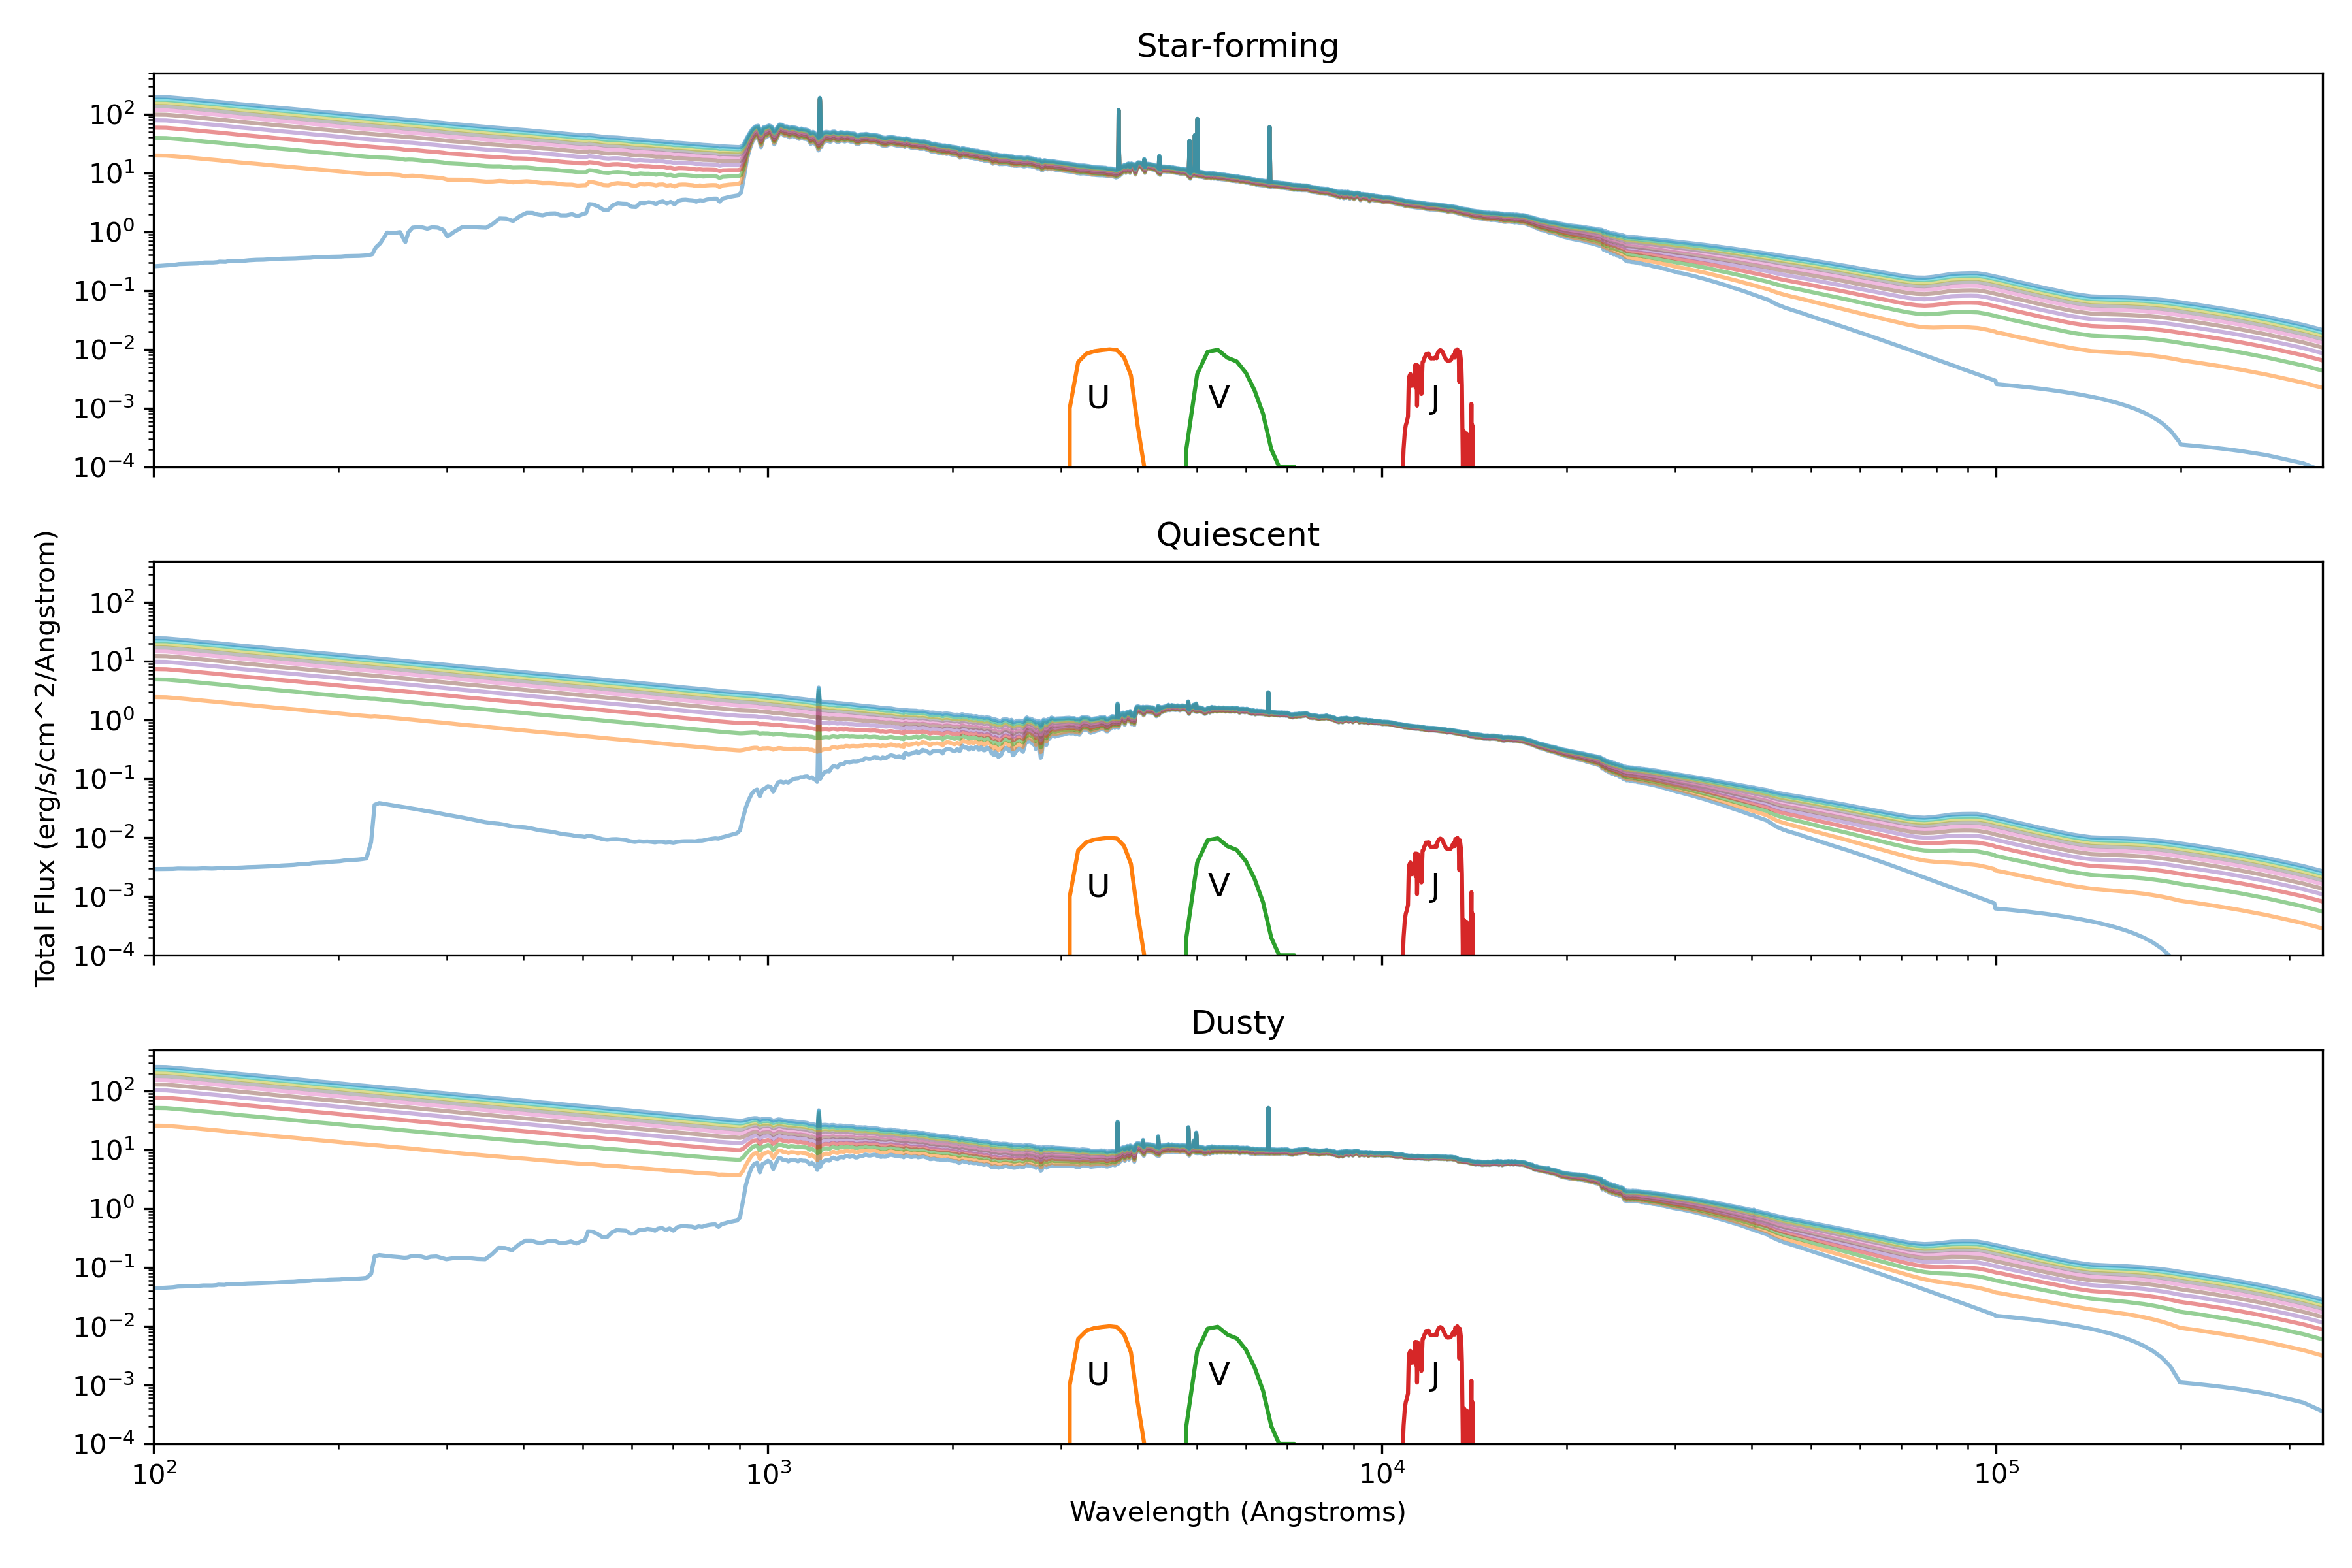
\includegraphics[width=1\linewidth]{Images//TheoreticalModelPlots/CompositeSEDs_UVJ.png}
    \caption{Rest frame Type 1 AGN Composites for the average galaxy in each region of the UVJ diagram. The blue line at the bottom of each plot signifies the initial source with no AGN contribution added. Each coloured line above it progressively incorporates an additional 10\% of the AGN's contribution to the total SED, culminating in a 100\% AGN-dominated SED.}
    \label{fig:composite_uvj}
\end{figure} \\
By investigating the SED of average ugr galaxies across different redshift ranges, we see how these galaxies vary, as redshift affects the observed colours in the ugr filter system. Figure \ref{fig:composite_ugr} illustrates how galaxy SEDs evolve with redshift. The ugr colour space is particularly valuable for identifying high-redshift galaxies, as it exploits the Lyman break – a sharp drop in flux in the u filter caused by absorption of ultraviolet light by neutral hydrogen – to pinpoint these distant objects. This characteristic drop is observed in our target redshift range, validating the effectiveness of this selection technique. The increase in AGN contribution ultimately causes an increase of flux within the range sampled by the u filter. Likewise, in the high redshift range, we see that both the u and g filters have experienced a drop in flux that increases with increased AGN contribution. Finally, by inspecting the lower redshift range, we see no noticeable difference with changing AGN contribution; additionally, as the redshift of the galaxy is too low, exploiting the dropout of flux from the u filter will not work, and thus, there will be no change to the selection region.
\begin{figure}[h!]
    \centering
    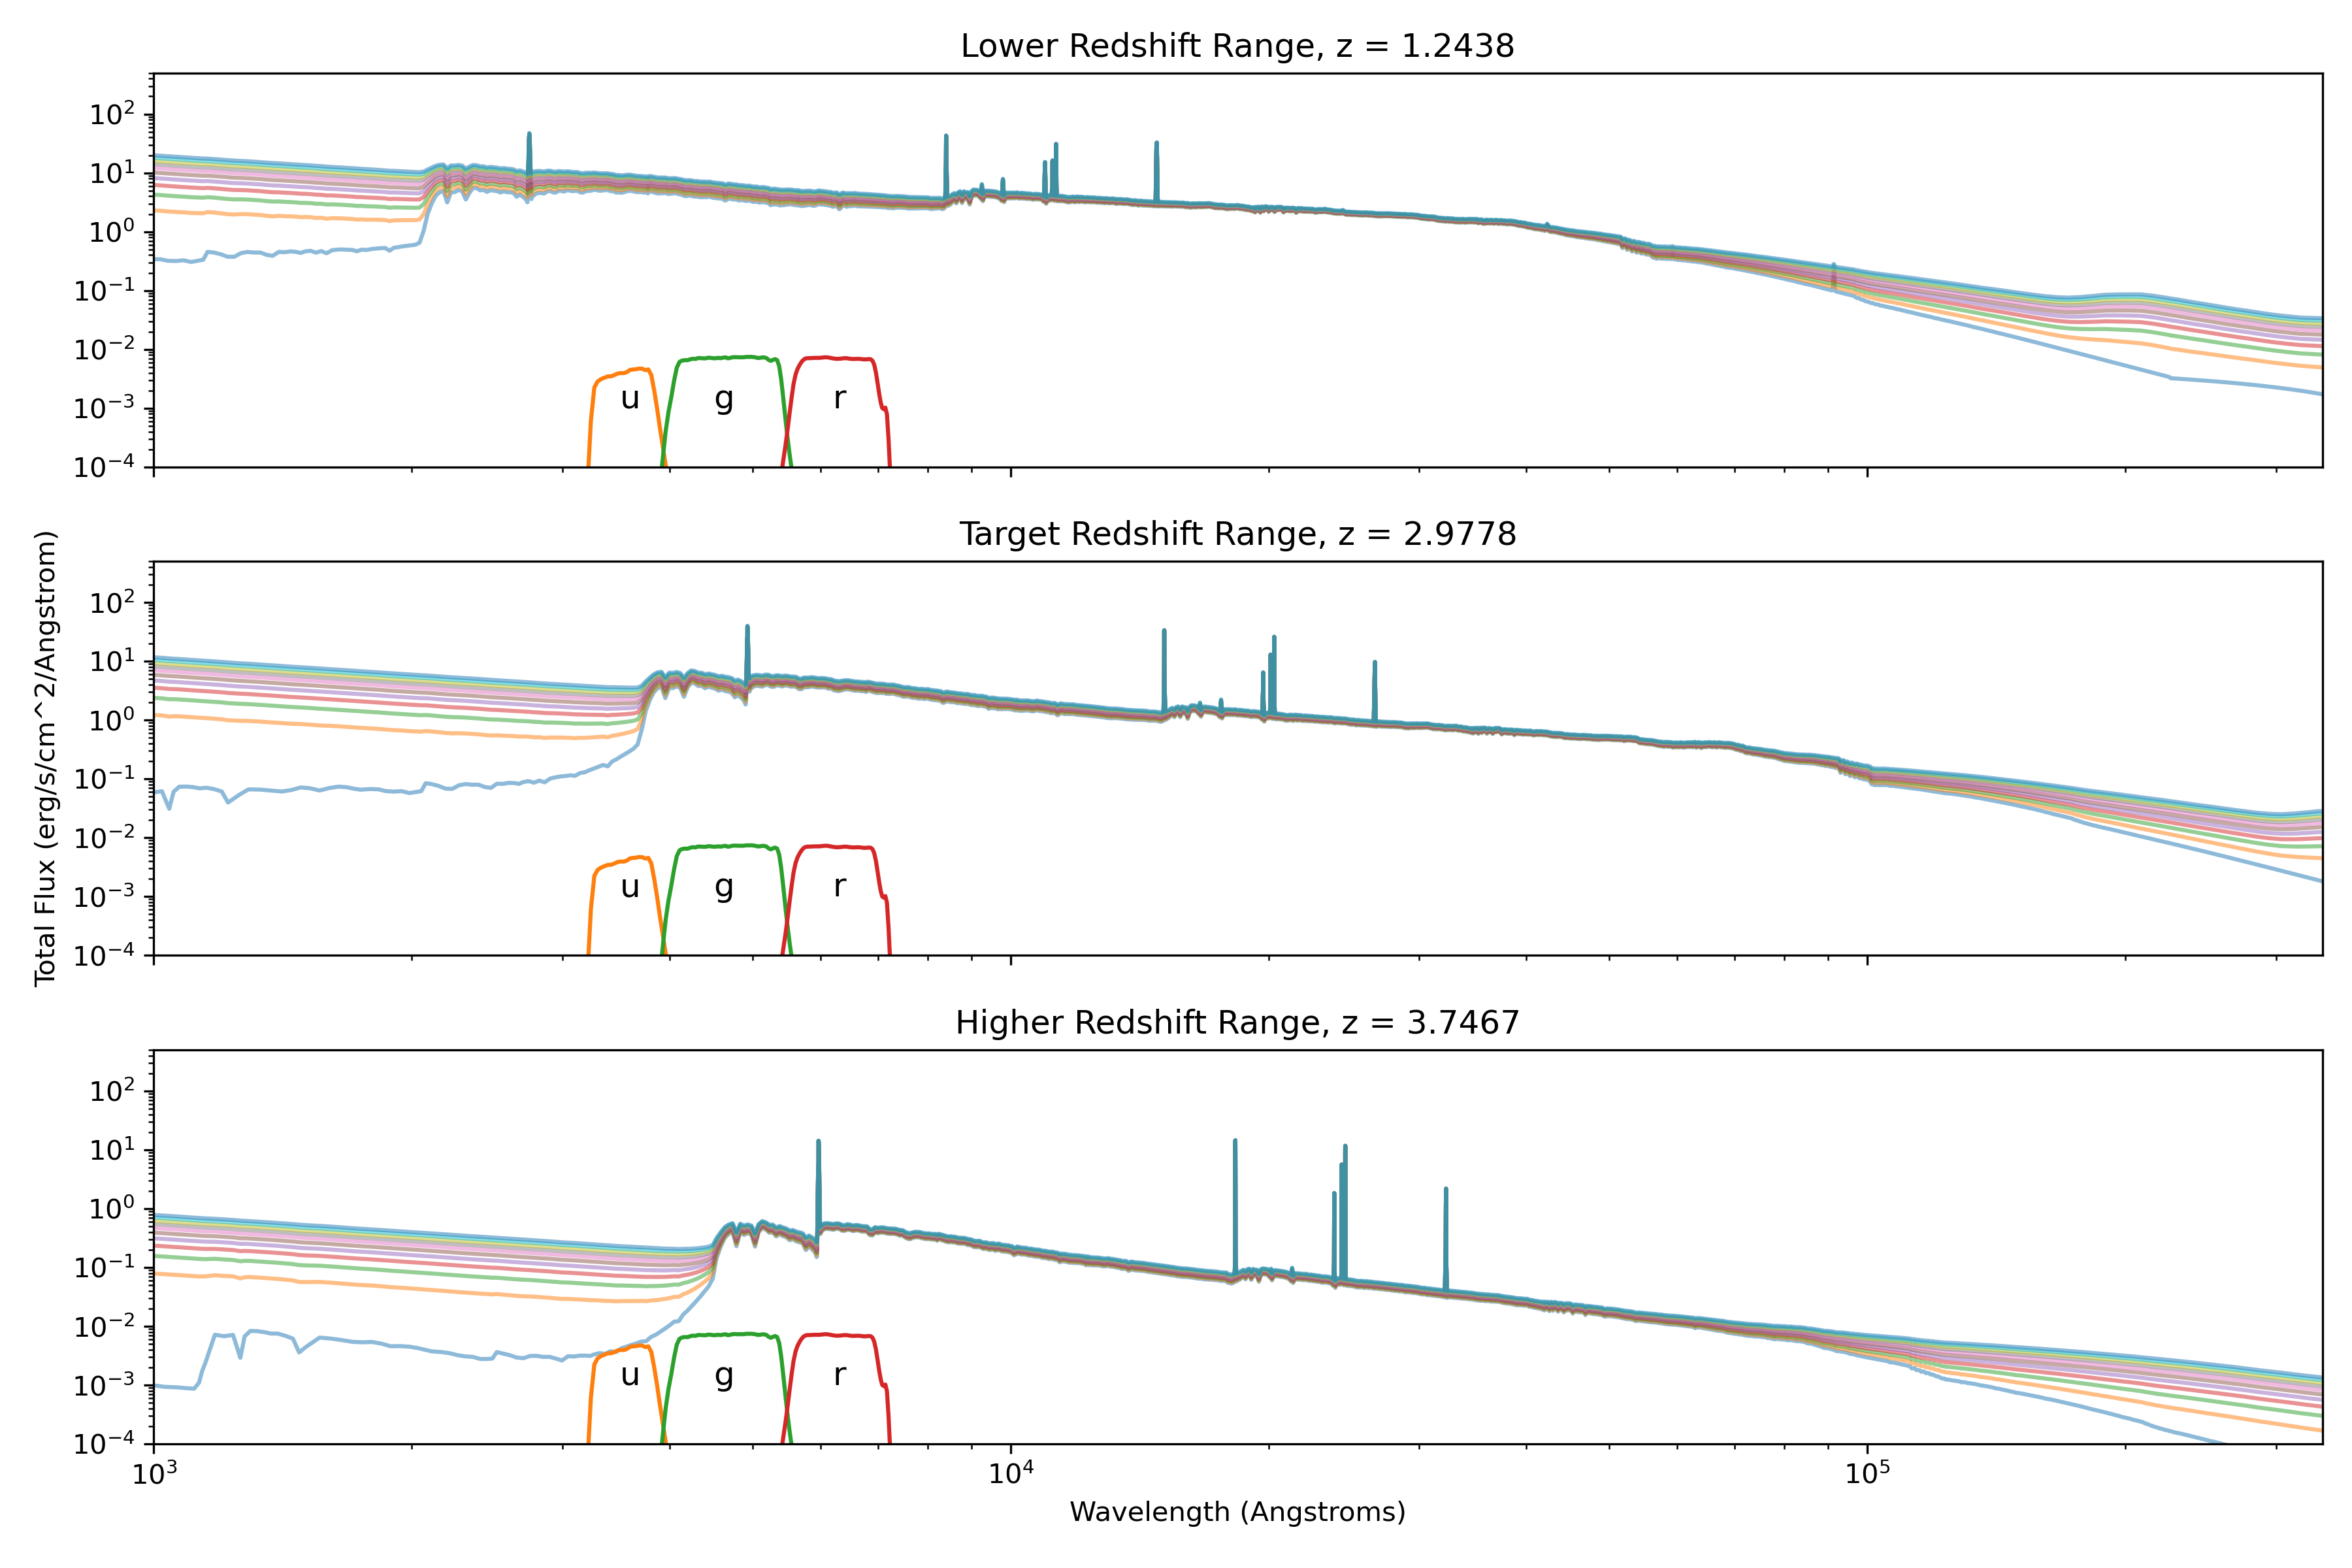
\includegraphics[width=1\linewidth]{Images//TheoreticalModelPlots/CompositeSEDs_ugr.png}
    \caption{Type 1 AGN Composites for the average galaxy in each redshift range of the ugr diagram. The blue line at the bottom of each plot represents the host galaxy's SED without any contribution from the AGN. }
    \label{fig:composite_ugr}
\end{figure}
\newpage
\subsection{CIGALE}
By using CIGALE, we can see the effect of SED decomposition on the sources in ZFOURGE. The results of SED decomposition and the resulting UVJ and ugr colour plots are presented in this section. A unique trait of the plots produced using CIGALE data is the striations present in the colourspace (See Figure \ref{fig:uvj-cigale-comparison}). While it is unknown what is causing these striations, it is suspected to be model degeneracy in the fitting process. However, possible reasons will be explored in the discussion of this work. In Figure\ref{fig:uvj-cigale-comparison}, we see that removing the AGN component causes a noticeable increase in the quiescent fraction and a proportionate decrease in the star-forming fraction, a behaviour observed in the previous two sections. 
\begin{figure}[h!]
    \centering
    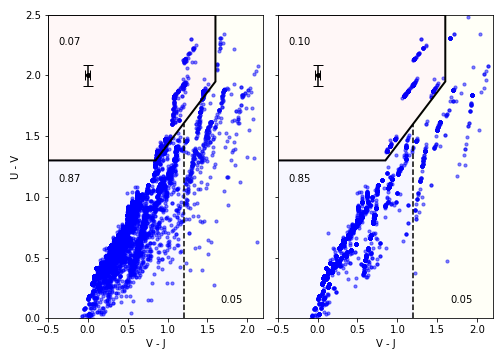
\includegraphics[width=0.75\linewidth]{Images/TheoreticalModelPlots/UVJ_agn_evolution_CIGALE_ZFOURGE_comparison.png}
    \caption{UVJ Diagram showing the full galaxy colours (left) and the decomposed colours that do not include AGN light (right). Error bars have been propagated from the original ZFOURGE survey.}
    \label{fig:uvj-cigale-comparison}
\end{figure}
Removing the AGN component revealed a noticeable shift in the colours of the sources. Sources that did not exhibit movement after decomposition (indicating the absence of an AGN) were excluded to isolate this effect. This allowed for a clearer visualisation of the general direction of these colour shifts (See Figure \ref{fig:decomposed-shift}).
\begin{figure}[h!]
    \centering
    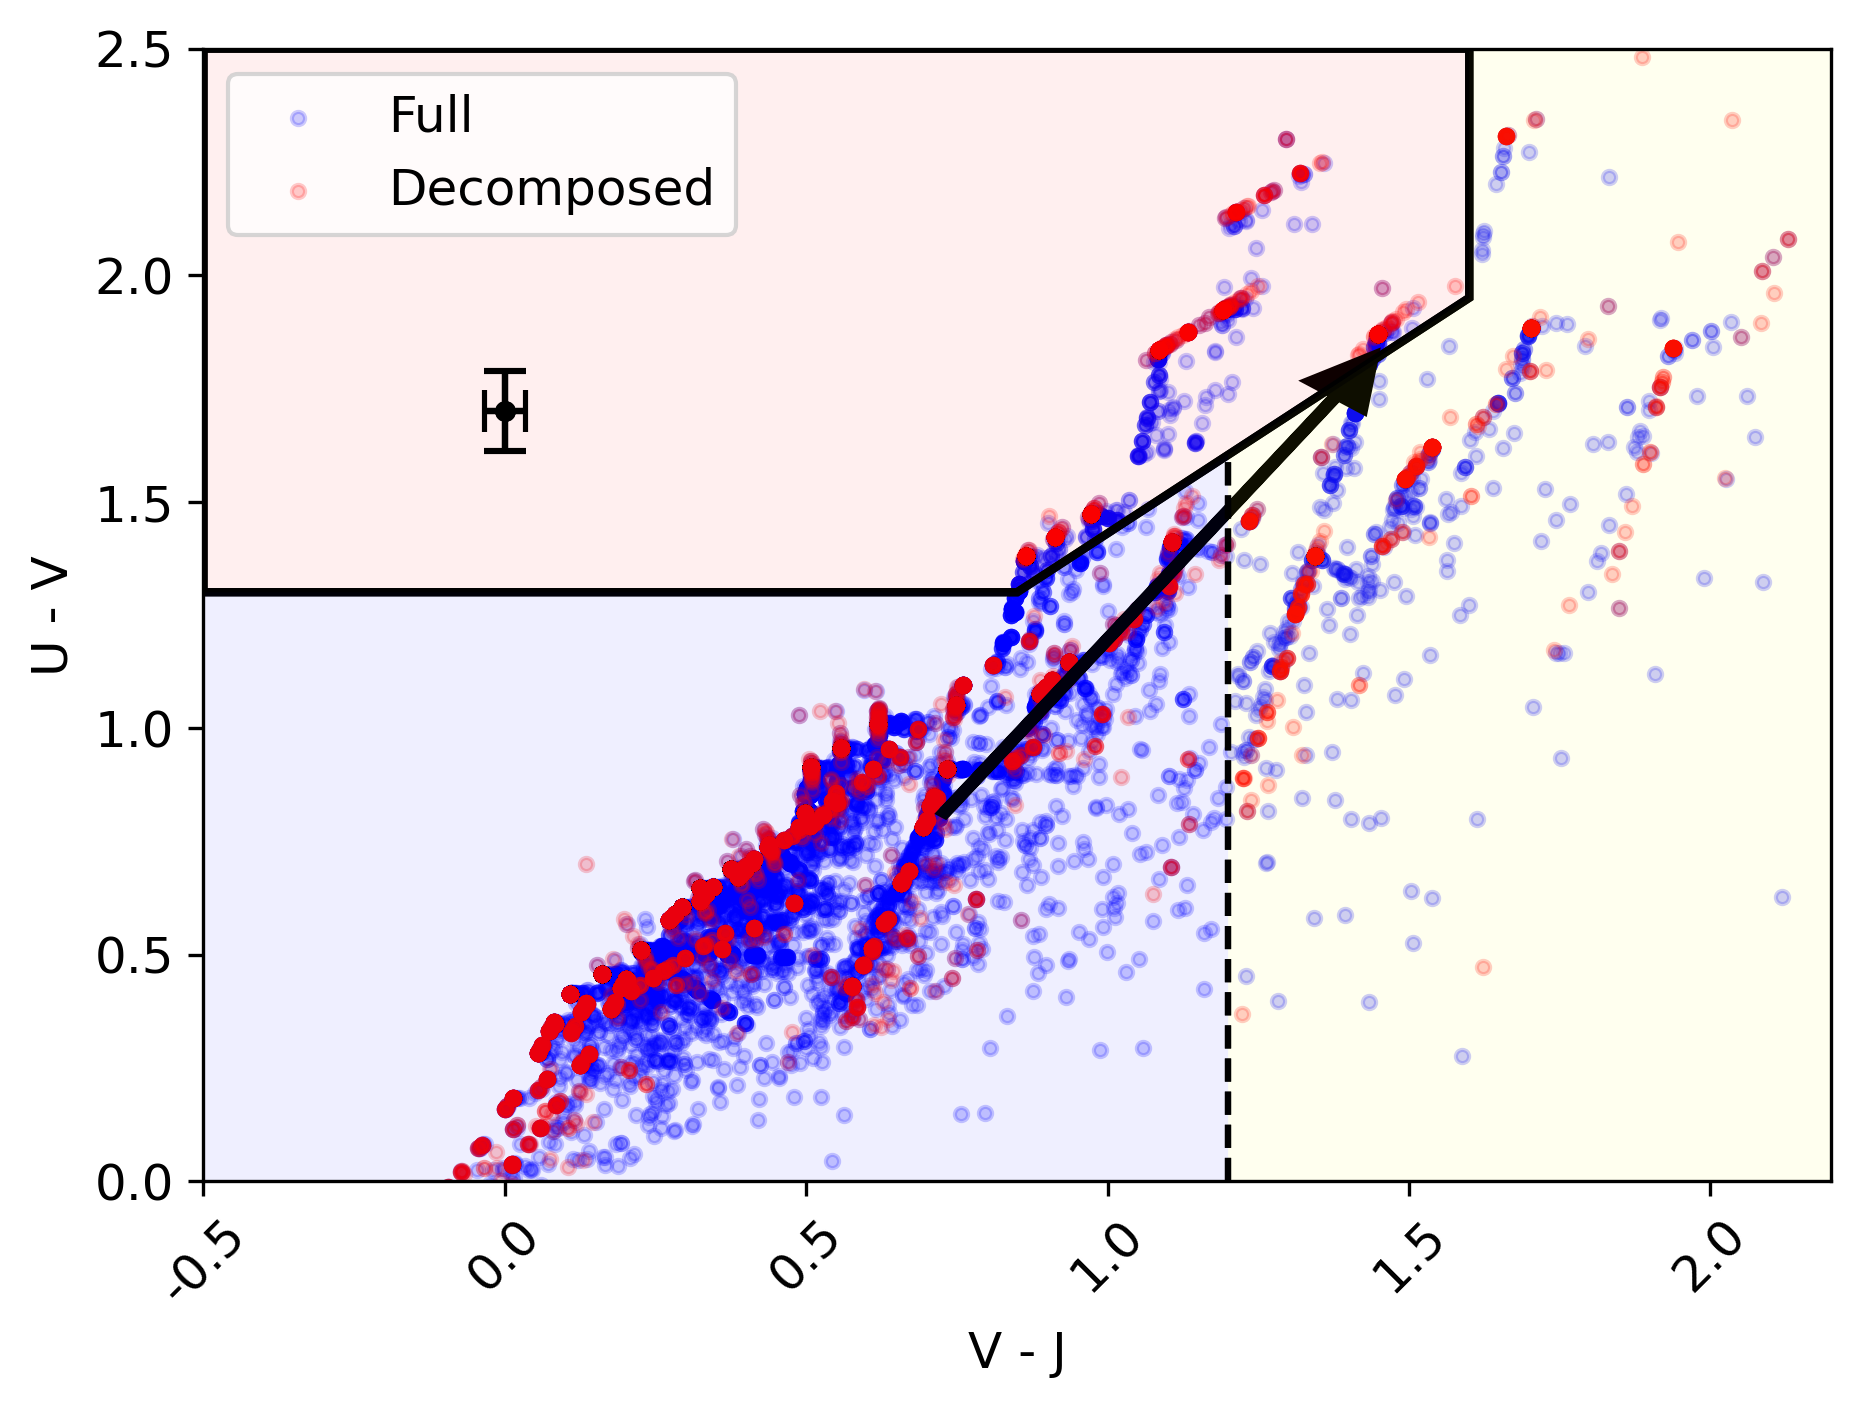
\includegraphics[width=0.75\linewidth]{Images/TheoreticalModelPlots/UVJ_agn_evolution_CIGALE_ZFOURGE_single_comparative.png}
    \caption{Full and Decomposed colours in the UVJ Diagram. The arrow indicates the general direction of the colour shift from the highest density region within the star-forming region. Note that the arrow's size does not represent the shift's magnitude.}
    \label{fig:decomposed-shift}
\end{figure}\newpage We also explore the redshift dependence of this decomposition process to investigate if the redshift evolution is affected by the removal of the AGN component. Figure \ref{fig:redshift-comparison} shows the average UVJ point throughout different redshift bins, both with and without an AGN component. We can see from the figure that both the complete UVJ colours and the decomposed UVJ colours share similar positions at low redshifts but begin to diverge at a redshift bin of 1.4 to -2, with the effect becoming more prominent at redshifts greater than 2. 
\begin{figure}[h!]
    \centering
    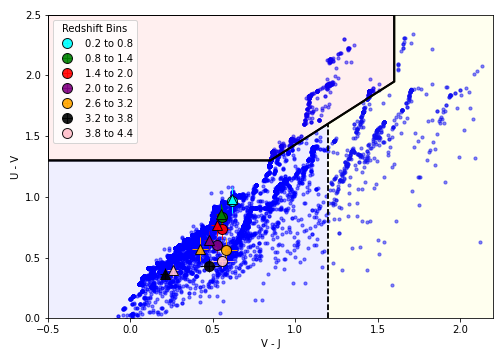
\includegraphics[width=0.7\linewidth]{Images/TheoreticalModelPlots/UVJ_agn_evolution_CIGALE_ZFOURGE_comparison_redshift.png}
    \caption{The UVJ Diagram shows a scatter plot of all sources. In this plot, the average location for each redshift bin is plotted. The full galaxies that include their AGN component are plotted as circles, while the decomposed galaxies that have their AGN removed have been plotted as triangles. Errors have been averaged for each redshift from all sources and propagated from the error in ZFOURGE.}
    \label{fig:redshift-comparison}
\end{figure}\\
Lastly, ugr diagrams were also created (See Figure \ref{fig:ugr-diagram-decomposed}). However, a full set of colour calculations for this colour space were unsuccessful, and thus, the outputs are somewhat incomplete. This is evidenced by almost all of the points in the high redshift bin missing. While this may be the case, this plot does show that introducing an AGN component into a colourspace reduces the completeness but may also result in less contamination from other undesirable sources within the selection area. This diagram did not include photometric errors since the colour space calculations failed.
\begin{figure}[h!]
    \centering
    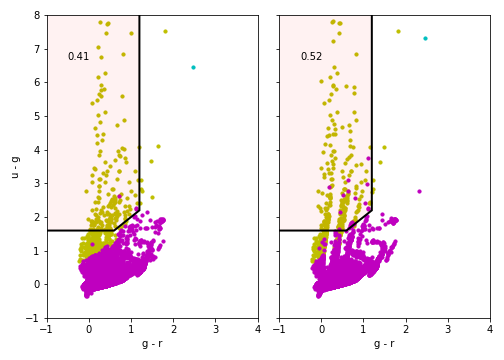
\includegraphics[width=0.8\linewidth]{Images/TheoreticalModelPlots/UGR_agn_evolution_CIGALE_ZFOURGE_comparison.png}
    \caption{The ugr plot shows both the decomposed galaxies (left), and the galaxies, which include their AGN component (right). The colour calculations for this plot failed; thus, there are few high redshift galaxies present within this plot.}
    \label{fig:ugr-diagram-decomposed}
\end{figure}
